\appendix 

\section{Experiment results} \label{app:results}

\begin{figure}[h!] 
	\begin{subfigure}[b]{\textwidth}		
		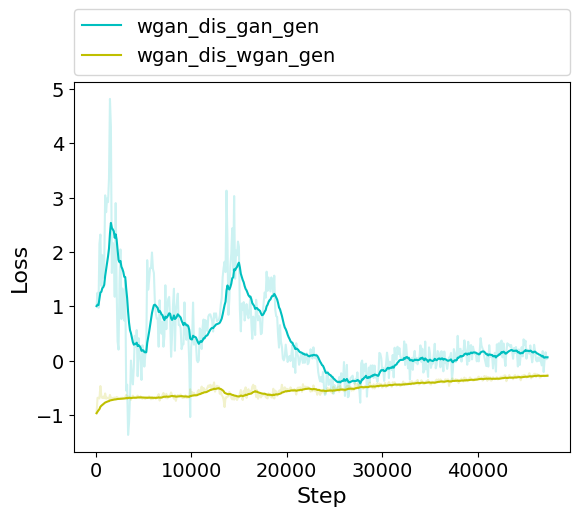
\includegraphics[width=0.5\textwidth]{figures/cross_dis/trial19_wgan_dis_gan_gen}
		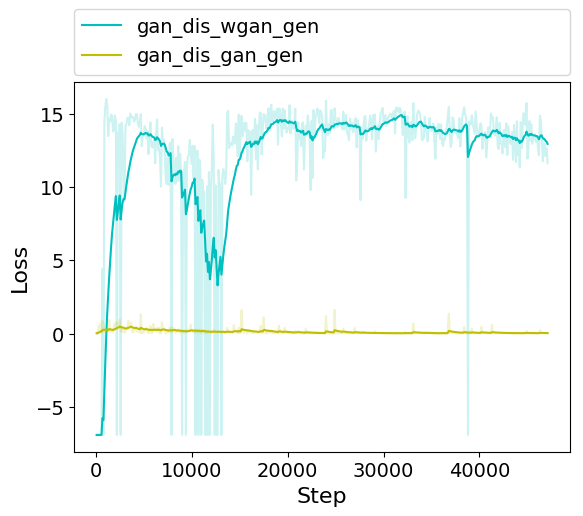
\includegraphics[width=0.5\textwidth]{figures/cross_dis/trial19_gan_dis_wgan_gen}
	\end{subfigure}
	\begin{subfigure}[b]{\textwidth}		
		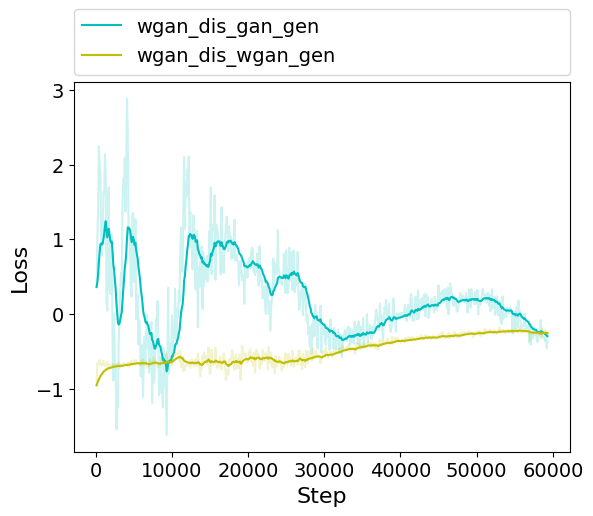
\includegraphics[width=0.5\textwidth]{figures/cross_dis/trial18_wgan_dis_gan_gen}
		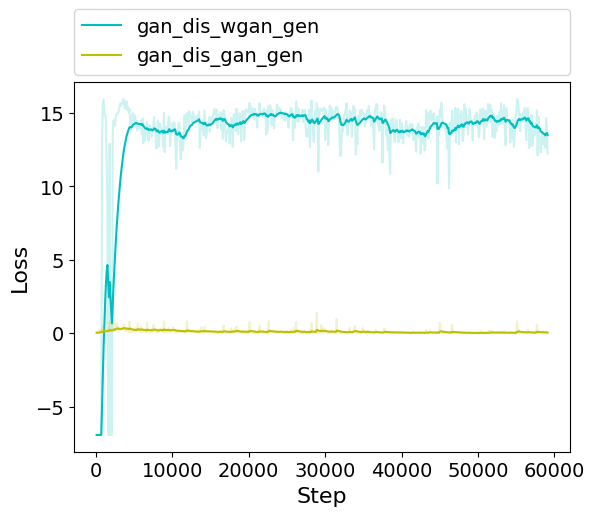
\includegraphics[width=0.5\textwidth]{figures/cross_dis/trial18_gan_dis_wgan_gen}
	\end{subfigure}
	\begin{subfigure}[b]{\textwidth}		
		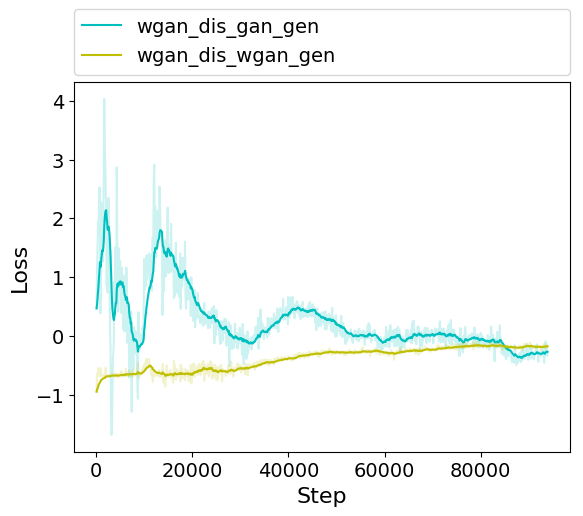
\includegraphics[width=0.5\textwidth]{figures/cross_dis/trial16_wgan_dis_gan_gen}
		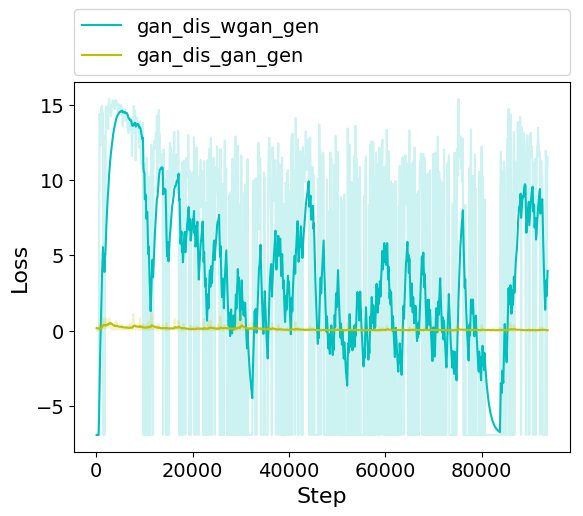
\includegraphics[width=0.5\textwidth]{figures/cross_dis/trial16_gan_dis_wgan_gen}
	\end{subfigure}
		\caption{A WGAN vs a GAN. The GAN discriminator's loss values are plotted using the logarithmic scale.}
\end{figure}

\begin{figure}[h!] 
	\begin{subfigure}[b]{\textwidth}		
		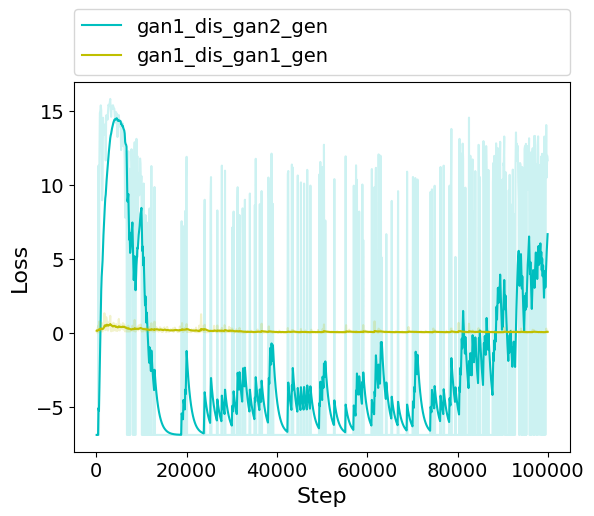
\includegraphics[width=0.5\textwidth]{figures/cross_dis/trial15_gan1_dis_gan2_gen}
		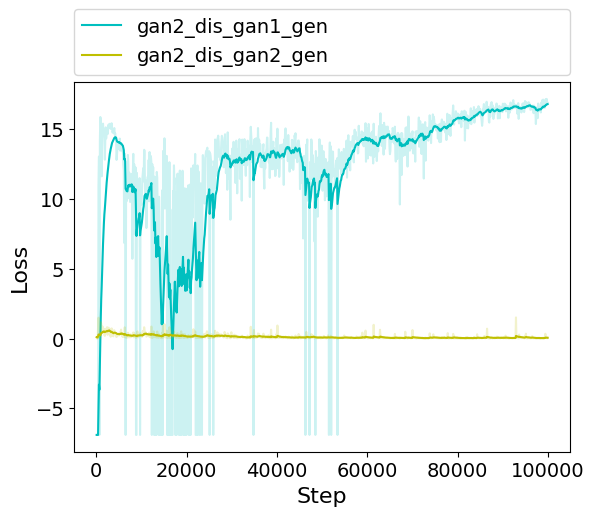
\includegraphics[width=0.5\textwidth]{figures/cross_dis/trial15_gan2_dis_gan1_gen}
	\end{subfigure}
	\begin{subfigure}[b]{\textwidth}		
		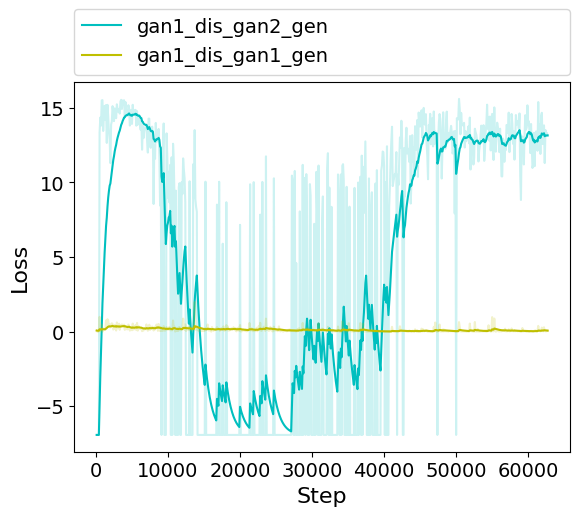
\includegraphics[width=0.5\textwidth]{figures/cross_dis/trial14_gan1_dis_gan2_gen}
		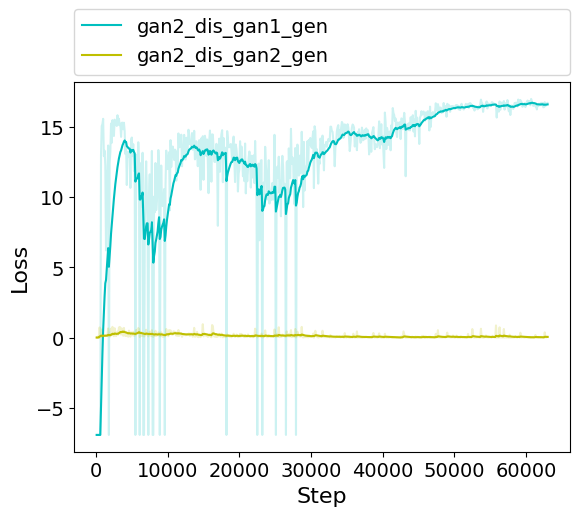
\includegraphics[width=0.5\textwidth]{figures/cross_dis/trial14_gan2_dis_gan1_gen}
	\end{subfigure}
	\caption{A GAN vs another GAN. Loss values are plotted using the logarithmic scale.}
\end{figure}

\begin{figure}[h!] 
	\begin{subfigure}[b]{\textwidth}		
		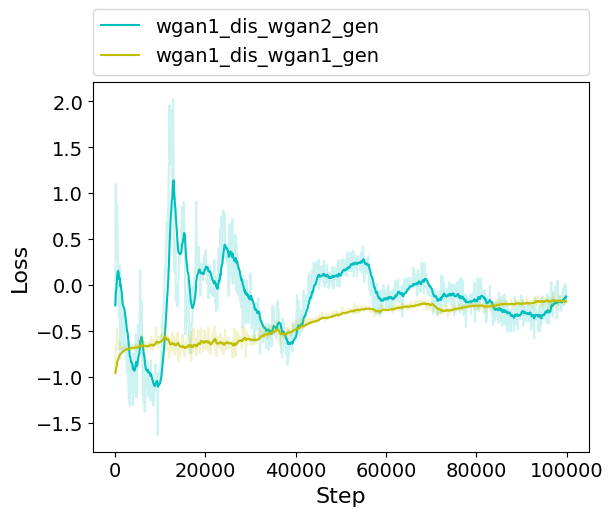
\includegraphics[width=0.5\textwidth]{figures/cross_dis/trial17_wgan1_dis_wgan2_gen}
		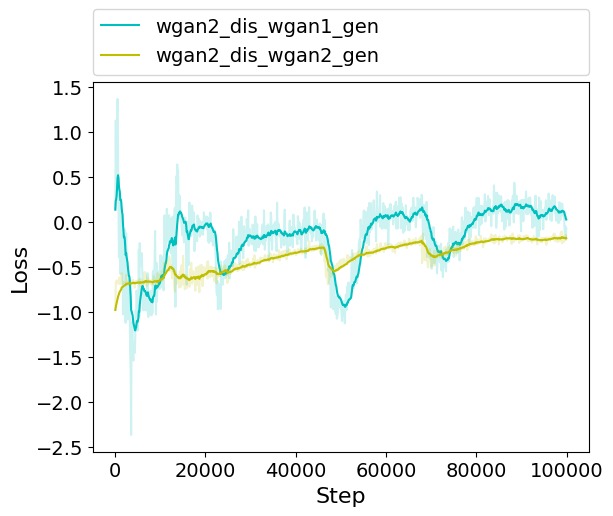
\includegraphics[width=0.5\textwidth]{figures/cross_dis/trial17_wgan2_dis_wgan1_gen}
	\end{subfigure}
	\caption{A WGAN vs another WGAN.}
\end{figure}

\begin{figure}[h]
	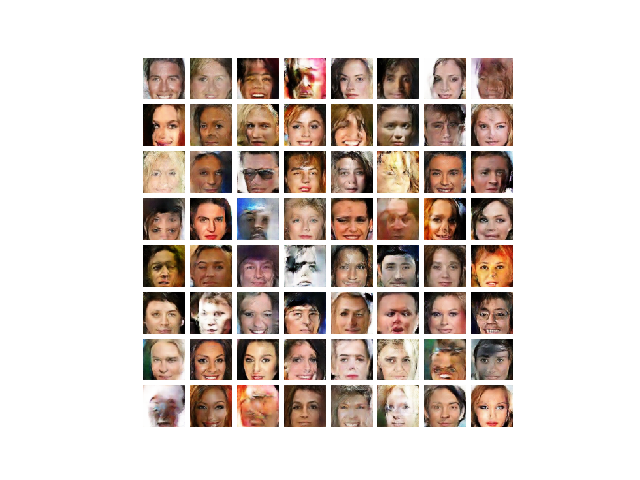
\includegraphics[scale=1.0]{figures/wgan_palette}
	\caption{Sample images produced by a WGAN generator}
\end{figure}


\begin{figure}[h]
	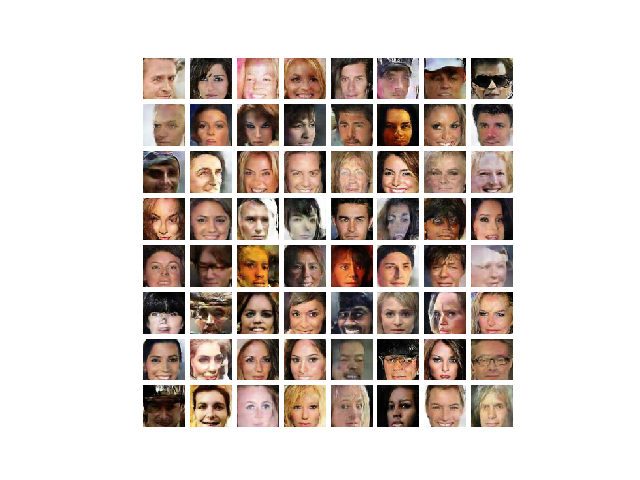
\includegraphics[scale=1.0]{figures/gan_palette}
	\caption{Sample images produced by a GAN generator}
\end{figure}